%%%%%%%%%%%%%%%%%%%%%%%%%%%%%%%%%%%%%%%%%%%%%%%%%%%%%%%%%%%%%%%%%%%%%%%%%%%%%%%%
% Troubleshooting
%%%%%%%%%%%%%%%%%%%%%%%%%%%%%%%%%%%%%%%%%%%%%%%%%%%%%%%%%%%%%%%%%%%%%%%%%%%%%%%%
\part{Troubleshooting} \label{Troubleshooting}

%%%%%%%%%%%%%%%%%%%%%%%%%%%%%%%%%%%%%%%%%%%%%%%%%%%%%%%%%%%%%%%%%%%%%%%%%%%%%%%%
% Common Issues
%%%%%%%%%%%%%%%%%%%%%%%%%%%%%%%%%%%%%%%%%%%%%%%%%%%%%%%%%%%%%%%%%%%%%%%%%%%%%%%%
\chapter{Common Issues} \label{Common Issues}

The following table lists common issues, their severity and possible
resolutions.

\ers{5}
\begin{longtabu} { X[5,l,m] | X[2,c,m] | X[7,l,m] }
  \thrule

  \thbi{Problem} & \thbi{Severity} & \thbi{Solution} \\ \mdrule

  Speakers pop when turning the \mAu{f} on.
    & \sNormal{sym}
    & Turn the \cVo{f} down before turning the \mAu{f} on. \\ \mrule

  The \cDi{f} shows remnants when switched \sOn{f}.
    & \sNormal{sym}
    & The \cDi{f} is getting power initially before it can display what
      it should. \\ \mrule

  The \cLB{f} flickers.
    & \sNormal{sym}
    & Try turning the \cVo{f} down and recharge.
      See \hyperref[Low Battery Indicator]{Low Battery Indicator}
      and \hyperref[Powering and Recharging]{Powering \& Recharging}. \\ \mrule

  You see \symD{OFF!} displayed but didn't do anything.
    & \sNormal{sym}
    & The \mAl{f} was turned off due to \textit{Wake Time} exceeded or
      \textit{Total Alarm Time} exceeded. \\ \mrule

  \pagebreak
  \mrule

  \multirow{3}{*}[-14mm]{\parbox{\linewidth}{You try to play a track and hear nothing.}}
    & \sLow{sym}
    & Try turning the \cVo{f} up. \\ \dcrule{2}{3}
  & \sMedium{sym}
    & \parbox{\linewidth}{\par\bigskip There may be a file that for some reason is
      unreadable.\footnote{ It could be that though the file has the correct extension,
      it isn't actually the type of file the extension would indicate.} Try
      picking another track.  If multiple tracks don't play then it may be a
      problem with the \cMSD{f} - see below. \par\bigskip} \\ \dcrule{2}{3}
  & \sHigh{sym}
    & The \cMSD{f} is formatted incorrectly or has failed.  See
    \hyperref[Removing SD Card]{Removing the Micro SD Card} for more
    information. \\ \mrule

  An error code and string are shown on the \cDi{f}.
    & \sHigh{sym}
    & See the \hyperref[Error Codes]{Errors} section. \\

  \bhrule
\caption{Troubleshooting Common Issues}
\end{longtabu}

%%%%%%%%%%%%%%%%%%%%%%%%%%%%%%%%%%%%%%%%%%%%%%%%%%%%%%%%%%%%%%%%%%%%%%%%%%%%%%%%
% Errors
%%%%%%%%%%%%%%%%%%%%%%%%%%%%%%%%%%%%%%%%%%%%%%%%%%%%%%%%%%%%%%%%%%%%%%%%%%%%%%%%
\chapter{Errors} \label{Error Codes}

Listed below are all of the possible errors that the device can recognize.  In
the event that you see one show up on the \cDi{f}, try the following.

\begin{itemize}
  \item \aTu{f} or \aPr{f} the \cEs{f} or \aTu{f} the \cRs{f} or fiddle with
    some other control on the \cFr{f} or \aTo{f} the \cTo{f} if the \cTS{f} is
    enabled.
\end{itemize}

If the error on the \cDi{f} doesn't go away or the problem continues to persist:

\begin{itemize}
  \item Switch the device \sOff{f} then back \sOn{f} using the \cPo{f}.
\end{itemize}

Again, if the error doesn't go away or the problem continues to persist, refer
to the following sections.

\info{If you are unable to resolve the problem or the device is unusable because
of the problem, please send the device back for repair.  Almost every part is
replaceable.}

\ers{3}
\begin{longtabu} { X[1,c,m] | X[1,c,m] | X[4,l,m] | }
  \thrule

  \thbi{Error Code} & \thbi{Error String} & \thbi{Description} \\ \mrule

  \sDl{!!!1}
    & \sDl{C.SEL.}
    & Problem with the \cRs{f}. \\ \mrule

  \sDl{!!!2}
    & \sDl{C.SEt.}
    & Problem with the \cEs{f}. \\ \mrule

  \sDl{!!!3}
    & \sDl{C.br.!}
    & Problem with the \cBr{f}. \\ \mrule

  \sDl{!!!4}
    & \sDl{C.PLA.}
    & Problem with \cPl{f} push-button. \\ \mrule

  \sDl{!!!5}
    & \sDl{C.nE.!}
    & Problem with \cNe{f} push-button. \\ \mrule

  \sDl{!!!6}
    & \sDl{C.PrE.}
    & Problem with \cPr{f} push-button. \\ \mrule

  \sDl{!!!7}
    & \sDl{BEEP}
    & Problem with the \cBe{f}. \\ \mrule

  \sDl{!!!8}
    & \sDl{dISP.}
    & Problem with the \cDi{f} - may not show. \\ \mrule

  \sDl{!!!9}
    & \sDl{LEdS}
    & Problem with the \cLi{f}. \\ \mrule

  \sDl{!!10}
    & \sDl{tUCH}
    & Problem with the \cTS{f}. \\ \mrule

  \sDl{!!11}
    & \sDl{FILE}
    & Problem with the \cMSD{f} or filesystem on the \cMSD{f}. \\ \mrule

  \sDl{!!12}
    & \sDl{Aud.!}
    & Problem with audio decoder or amplifier. \\ \mrule

  \sDl{!!13}
    & \sDl{PLAY}
    & The \mAu{f} is disabled. \\ \mrule

  \sDl{!!14}
    & \sDl{P.FIL.}
    & Problem obtaining audio files from the \cMSD{f}. \\ \mrule

  \sDl{!!15}
    & \sDl{P.OPE.}
    & Problem opening an audio file on the \cMSD{f}. \\ \mrule

  \sDl{!!16}
    & \sDl{P.Aud.}
    & Problem communicating with audio decoder or reading a file. \\ \mrule

  \sDl{!!17}
    & \sDl{T.PIt.}
    & Problem getting access to timer. \\

  \bhrule
\caption{Error Codes}
\end{longtabu}

\section{Hardware}

This class of error indicates a problem with the hardware.  There are a
few possibilities as to the cause:

\begin{enumerate}
  \item The named piece of hardware has failed.
  \item The microcontroller has failed.
  \item The \textit{connection} between the named piece of hardware and
    microcontroller has been severed.  This could be a due to a couple
    or reasons:
    \begin{itemize}
      \item A cable that connects the named piece of hardware to the
        circuit board is disconnected or severed, \textit{or}
      \item A solder connection or trace on the circuit board has gone bad.
    \end{itemize}
  \item The named piece of hardware is actually working which likely points to a
    bug in the software.
\end{enumerate}

It is also possible that a piece of hardware could be malfunctioning without
any error showing up on the \cDi{f}.

%%%%%%%%%%%%%%%%%%%%%%%%%%%%%%%%%%%%%%%%%%%%%%%%%%%%%%%%%%%%%%%%%%%%%%%%%%%%%%%%
% Controls
%%%%%%%%%%%%%%%%%%%%%%%%%%%%%%%%%%%%%%%%%%%%%%%%%%%%%%%%%%%%%%%%%%%%%%%%%%%%%%%%
\subsection{Controls}

If there is a problem with one of the controls, first check to see if the
cable connecting the control to the circuit board is disconnected or severed.
Refer to \hyperref[Disassembly]{Disassembly} for instructions on removing the
\cTo{f}.

%%%%%%%%%%%%%%%%%%%%%%%%%%%%%%%%%%%%%%%%%%%%%%%%%%%%%%%%%%%%%%%%%%%%%%%%%%%%%%%%
% Controls - Selector Dial
%%%%%%%%%%%%%%%%%%%%%%%%%%%%%%%%%%%%%%%%%%%%%%%%%%%%%%%%%%%%%%%%%%%%%%%%%%%%%%%%
\subsubsection{Selector Dial}

\sD{!!!1} \sD{C.SEL.}

\par\bigskip

The side of the cable that is connected to the \cRs{f} is soldered.  There
are \num{4} connections to the \cRs{f}.  If any one of these is disconnected
then the problem is likely one of connection and \textit{not} due to the
\cRs{f} itself being broken.

\par\medskip

The side of the cable that is connected to the circuit board is a very secure
connection, however, it is possible that a solder joint that connects the
female connector to the circuit board has failed.

%%%%%%%%%%%%%%%%%%%%%%%%%%%%%%%%%%%%%%%%%%%%%%%%%%%%%%%%%%%%%%%%%%%%%%%%%%%%%%%%
% Controls - Settings Knob
%%%%%%%%%%%%%%%%%%%%%%%%%%%%%%%%%%%%%%%%%%%%%%%%%%%%%%%%%%%%%%%%%%%%%%%%%%%%%%%%
\subsubsection{Settings Knob} \label{Errors - Settings Knob}

\sD{!!!2} \sD{C.SEt.}

\par\bigskip

The cable connecting the \cEs{f} is terminated with a connector that slides
over the pins of the \cEs{f}.  If this is disconnected, try reconnecting it.
The figure below shows how the cable should be oriented, with the
\textit{red} cable on the \textit{bottom}.

\begin{figure}[H]
\centering
  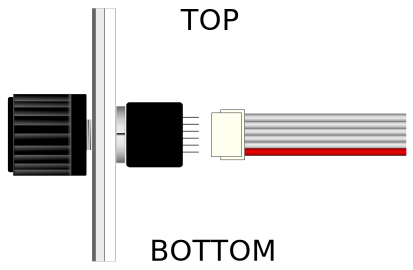
\includegraphics{images/rotary_encoder.png}
\caption{Settings Knob and Brightness Knob Cable Alignment} \label{fig:Encoder Cable}
\end{figure}

\par\medskip

The side of the cable that is connected to the circuit board is a very secure
connection, however, it is possible that a solder joint that connects the
female connector to the circuit board has failed.

\par\medskip

If the \cEs{f} responds to turning but \textit{not} to pressing, then the
problem may be due to the circuitry that does switch debouncing.

%%%%%%%%%%%%%%%%%%%%%%%%%%%%%%%%%%%%%%%%%%%%%%%%%%%%%%%%%%%%%%%%%%%%%%%%%%%%%%%%
% Controls - Brightness Knob
%%%%%%%%%%%%%%%%%%%%%%%%%%%%%%%%%%%%%%%%%%%%%%%%%%%%%%%%%%%%%%%%%%%%%%%%%%%%%%%%
\subsubsection{Brightness Knob}

\sD{!!!3} \sD{C.br.!}

\par\bigskip

The cable connecting the \cEs{f} is terminated with a connector that slides
over the pins of the \cEs{f}.  If this is disconnected, try reconnecting it.
See the \hyperref[fig:Encoder Cable]{Figure \ref*{fig:Encoder Cable}}
in \hyperref[Errors - Settings Knob]{Settings Knob} above for how the
cable should be aligned.

\par\medskip

The side of the cable that is connected to the circuit board is a very secure
connection, however, it is possible that a solder joint that connects the
female connector to the circuit board has failed.

%%%%%%%%%%%%%%%%%%%%%%%%%%%%%%%%%%%%%%%%%%%%%%%%%%%%%%%%%%%%%%%%%%%%%%%%%%%%%%%%
% Controls - Play | Pause | Stop
%%%%%%%%%%%%%%%%%%%%%%%%%%%%%%%%%%%%%%%%%%%%%%%%%%%%%%%%%%%%%%%%%%%%%%%%%%%%%%%%
\subsubsection{Play | Pause | Stop}

\sD{!!!4} \sD{C.PLA.}

\par\bigskip

The side of the cable that is connected to the \cPl{f} push-button is soldered.
There are \num{2} connections to the \cPl{f} push-button.  If any one of these
is disconnected then the problem is likely one of connection and \textit{not}
due to the \cPl{f} push-button itself being broken.

\par\medskip

The side of the cable that is connected to the circuit board is a very secure
connection, however, it is possible that a solder joint that connects the
female connector to the circuit board has failed.

\par\medskip

The problem may also be due to the circuitry that does switch debouncing.

%%%%%%%%%%%%%%%%%%%%%%%%%%%%%%%%%%%%%%%%%%%%%%%%%%%%%%%%%%%%%%%%%%%%%%%%%%%%%%%%
% Controls - Next
%%%%%%%%%%%%%%%%%%%%%%%%%%%%%%%%%%%%%%%%%%%%%%%%%%%%%%%%%%%%%%%%%%%%%%%%%%%%%%%%
\subsubsection{Next}

\sD{!!!5} \sD{C.nE.!}

\par\bigskip

The side of the cable that is connected to the \cNe{f} push-button is soldered.
There are \num{2} connections to the \cNe{f} push-button.  If any one of these
is disconnected then the problem is likely one of connection and \textit{not}
due to the \cNe{f} push-button itself being broken.

\par\medskip

The side of the cable that is connected to the circuit board is a very secure
connection, however, it is possible that a solder joint that connects the
female connector to the circuit board has failed.

\par\medskip

The problem may also be due to the circuitry that does switch debouncing.

%%%%%%%%%%%%%%%%%%%%%%%%%%%%%%%%%%%%%%%%%%%%%%%%%%%%%%%%%%%%%%%%%%%%%%%%%%%%%%%%
% Controls - Previous
%%%%%%%%%%%%%%%%%%%%%%%%%%%%%%%%%%%%%%%%%%%%%%%%%%%%%%%%%%%%%%%%%%%%%%%%%%%%%%%%
\subsubsection{Previous}

\sD{!!!6} \sD{C.PrE.}

\par\bigskip

The side of the cable that is connected to the \cPr{f} push-button is soldered.
There are \num{2} connections to the \cPr{f} push-button.  If any one of these
is disconnected then the problem is likely one of connection and \textit{not}
due to the \cPr{f} push-button itself being broken.

\par\medskip

The side of the cable that is connected to the circuit board is a very secure
connection, however, it is possible that a solder joint that connects the
female connector to the circuit board has failed.

\par\medskip

The problem may also be due to the circuitry that does switch debouncing.

%%%%%%%%%%%%%%%%%%%%%%%%%%%%%%%%%%%%%%%%%%%%%%%%%%%%%%%%%%%%%%%%%%%%%%%%%%%%%%%%
% Beeper
%%%%%%%%%%%%%%%%%%%%%%%%%%%%%%%%%%%%%%%%%%%%%%%%%%%%%%%%%%%%%%%%%%%%%%%%%%%%%%%%
\subsection{Beeper}

\sD{!!!7} \sD{BEEP}

\par\bigskip

The \cBe{f} is soldered directly to the circuit board.  If it is loose then
it's a problem of connection, otherwise it has failed.

%%%%%%%%%%%%%%%%%%%%%%%%%%%%%%%%%%%%%%%%%%%%%%%%%%%%%%%%%%%%%%%%%%%%%%%%%%%%%%%%
% Screens
%%%%%%%%%%%%%%%%%%%%%%%%%%%%%%%%%%%%%%%%%%%%%%%%%%%%%%%%%%%%%%%%%%%%%%%%%%%%%%%%
\subsection{Screens}

%%%%%%%%%%%%%%%%%%%%%%%%%%%%%%%%%%%%%%%%%%%%%%%%%%%%%%%%%%%%%%%%%%%%%%%%%%%%%%%%
% Screens - Display
%%%%%%%%%%%%%%%%%%%%%%%%%%%%%%%%%%%%%%%%%%%%%%%%%%%%%%%%%%%%%%%%%%%%%%%%%%%%%%%%
\subsubsection{Display}

\sD{!!!8} \sD{dISP.}

\par\bigskip

The \cDi{f} is actually working, at least in part, if you see this error.
It indicates a problem with the \textbf{I$^2$C} communication bus between the
\cDi{f} and the microcontroller.

\par\medskip

The cable connection to both the \cDi{f} and circuit board is are very
secure connections, however, it is possible that a solder joint that connects
the female connector to one or both has failed.

%%%%%%%%%%%%%%%%%%%%%%%%%%%%%%%%%%%%%%%%%%%%%%%%%%%%%%%%%%%%%%%%%%%%%%%%%%%%%%%%
% Screens - Lighting
%%%%%%%%%%%%%%%%%%%%%%%%%%%%%%%%%%%%%%%%%%%%%%%%%%%%%%%%%%%%%%%%%%%%%%%%%%%%%%%%
\subsubsection{Lighting}

\sD{!!!9} \sD{LEdS}

\par\bigskip

There are \num{2} rows of \num{8} LEDs in each row that make up the \cLi{f}.
Each row or strip is soldered to a small circuit board.  These connections
may be the problem for the failure.

\par\medskip

The cable connection to both the \cLi{f} and circuit board is are very
secure connections, however, it is possible that a solder joint that connects
the female connector to one or both has failed.

%%%%%%%%%%%%%%%%%%%%%%%%%%%%%%%%%%%%%%%%%%%%%%%%%%%%%%%%%%%%%%%%%%%%%%%%%%%%%%%%
% Touch Sensor
%%%%%%%%%%%%%%%%%%%%%%%%%%%%%%%%%%%%%%%%%%%%%%%%%%%%%%%%%%%%%%%%%%%%%%%%%%%%%%%%
\subsection{Touch Sensor}

\sD{!!10} \sD{tUCH}

\par\bigskip

There is a wire connecting the \cTS{f} to the microcontroller.  The terminal
connecting to the \cTS{f} is a ring terminal held in place by a screw.  Make
sure this is tight.

\par\medskip

Otherwise, the cable may be severed.

%%%%%%%%%%%%%%%%%%%%%%%%%%%%%%%%%%%%%%%%%%%%%%%%%%%%%%%%%%%%%%%%%%%%%%%%%%%%%%%%
% Filesystem or Micro SD Card
%%%%%%%%%%%%%%%%%%%%%%%%%%%%%%%%%%%%%%%%%%%%%%%%%%%%%%%%%%%%%%%%%%%%%%%%%%%%%%%%
\subsection{Filesystem or Micro SD Card}

\sD{!!11} \sD{FILE}

\par\bigskip

This could mean that either:

\begin{enumerate}
  \item The filesystem on the \cMSD{f} is not formatted as \mono{FAT32} with
    \num{512} bytes / sector, \textit{or}
  \item The filesystem is corrupted and/or the \cMSD{f} is bad.
\end{enumerate}

If you have just replaced the \cMSD{f}, it may mean that it was formatted
incorrectly.  If you haven't replaced the \cMSD{f}, then it will likely need
replacing.  Refer to \hyperref[Removing SD Card]{Removing the Micro SD Card}
for instructions.

%%%%%%%%%%%%%%%%%%%%%%%%%%%%%%%%%%%%%%%%%%%%%%%%%%%%%%%%%%%%%%%%%%%%%%%%%%%%%%%%
% Audio Decoder or Amplifier
%%%%%%%%%%%%%%%%%%%%%%%%%%%%%%%%%%%%%%%%%%%%%%%%%%%%%%%%%%%%%%%%%%%%%%%%%%%%%%%%
\subsection{Audio Decoder or Amplifier}

\sD{!!12} \sD{Aud.!}

\par\bigskip

This likely means that the audio decoder or amplifier has failed.

%%%%%%%%%%%%%%%%%%%%%%%%%%%%%%%%%%%%%%%%%%%%%%%%%%%%%%%%%%%%%%%%%%%%%%%%%%%%%%%%
% Audio
%%%%%%%%%%%%%%%%%%%%%%%%%%%%%%%%%%%%%%%%%%%%%%%%%%%%%%%%%%%%%%%%%%%%%%%%%%%%%%%%
\section{Audio}

These errors may or may not be recoverable and may or may not be hardware
issues.

%%%%%%%%%%%%%%%%%%%%%%%%%%%%%%%%%%%%%%%%%%%%%%%%%%%%%%%%%%%%%%%%%%%%%%%%%%%%%%%%
% Audio - Disabled
%%%%%%%%%%%%%%%%%%%%%%%%%%%%%%%%%%%%%%%%%%%%%%%%%%%%%%%%%%%%%%%%%%%%%%%%%%%%%%%%
\subsection{Audio Disabled}

\sD{!!13} \sD{PLAY}

\par\bigskip

This error indicates that the \mAu{f} has been \textit{disabled} due to one of
the following:

\begin{table}[H]
\ers{0.1}
\centering
\begin{tabu}{c}
  \symD{!!11} \symD{FILE} \\
  \symD{!!12} \symD{Aud.!} \\
  \symD{!!14} \symD{P.FIL.} \\
  \symD{!!15} \symD{P.OPE.} \\
  \symD{!!16} \symD{P.Aud.} \\
\end{tabu}
\end{table}

You will see one of the above errors \textit{first}, then this error indicating
that the \mAu{f} has been disabled and is unusable.

%%%%%%%%%%%%%%%%%%%%%%%%%%%%%%%%%%%%%%%%%%%%%%%%%%%%%%%%%%%%%%%%%%%%%%%%%%%%%%%%
% Audio - Files
%%%%%%%%%%%%%%%%%%%%%%%%%%%%%%%%%%%%%%%%%%%%%%%%%%%%%%%%%%%%%%%%%%%%%%%%%%%%%%%%
\subsection{Audio Files}

\par\bigskip

\begin{table}[H]
\ers{3.0}
\begin{tabu}{X[1,c,m] X[4,l,m]}
  \mrule
  \sD{!!14} \sD{P.FIL.}
    & There is a problem obtaining the audio files from the \cMSD{f}. \\ \drule{2}
  \sD{!!15} \sD{P.OPE.}
    & There is a problem opening an audio file that is on the the \cMSD{f}. \\ \drule{2}
  \sD{!!16} \sD{P.Aud.}
    & There is a problem communicating with the audio decoder or a problem
      reading an audio file that is on the the \cMSD{f}. \\
  \mrule
\end{tabu}
\end{table}

These are likely due to one of the following:

\begin{enumerate}
  \item The \cMSD{f} is not formatted correctly or is failing.
  \item There is a problem with the audio decoder.
\end{enumerate}

If you have just replaced the \cMSD{f}, it may mean that it was formatted
incorrectly.  If you haven't replaced the \cMSD{f}, then try replacing it.
Refer to \hyperref[Removing SD Card]{Removing the Micro SD Card} for
instructions.

\par\medskip

If the above doesn't solve the problem, then it likely means that the audio
decoder has failed.

%%%%%%%%%%%%%%%%%%%%%%%%%%%%%%%%%%%%%%%%%%%%%%%%%%%%%%%%%%%%%%%%%%%%%%%%%%%%%%%%
% Timer
%%%%%%%%%%%%%%%%%%%%%%%%%%%%%%%%%%%%%%%%%%%%%%%%%%%%%%%%%%%%%%%%%%%%%%%%%%%%%%%%
\section{Timer}

\sD{!!17} \sD{T.PIt.}

\par\bigskip

This error indicates that a timer could not be acquired.  It should
never happen and indicates a bug in the software.

